\section{Design and Implementation}\label{Design and Implementation}
	In this section we will discuss the design and implementation of the whole system. First of is the section about the client side of the equation and then follows the server side. 
	
	Below is a first taste of how our system works. In figure \ref{fig:totaloverview} you can see a cloud of clients which can be on the same local network or be on different networks. The \textit{ESB} talks to \textit{GlassFish} where services are placed and clients talk to the ESB which mediates the message into GlassFish. In order for the ESB to know how much bandwidth each client can utilize, it is dependent on the \textit{Monitoring Service} which relays that sort of network information.
    
    \begin{figure}[H]
        \centering
        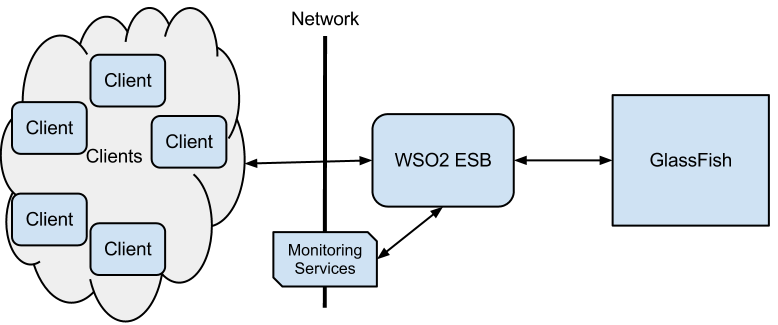
\includegraphics[scale=0.5]{Totaloverview}
        \caption{Total Overview}
        This figure shows roughly how our project looks from a bird's-eye view.
        \label{fig:totaloverview}
    \end{figure}

    \subsection{Client Side}\label{client side}

This chapter will introduce the design and architecture of the client side of our system. Section \ref{client introduction} will introduce the different components that make up the entire client, and includes a description of the different components that make up the client library. Next, section \ref{client use cases} will describe the use cases, and section \ref{textual client data flow} will take care of the data flow, followed by a detailed architecture description \ref{client architecture}. Finally, section \ref{client sequence diagrams} will go through the sequence diagrams.
    
    The class diagram is a usefull addition when understanding the architecture of the client library and it's functionality. The descriptions and diagrams in this section might become clearer when looking at the class diagram and see the connections between classes and the more specific contents of the classes. 
		
    \subsubsection{Introduction}\label{client introduction}
The client architecture consists of the following components: The client application, the client library and the Monitoring Service. Additionally, the library makes use of some external components to do some of it's work.

    \subsubsection{Component description:}\label{Component description}

\indent \indent \textbf{Client application:}\\
	The user-controlled applications that utilize web services. These must be modified to send all communication through the client library in order to get the prioritization it should have.
\\\\

\indent \textbf{Client library:}\\
% needs to be rewritten and clearified. 
This component will handle all communication with the service providers, as well as authenticating users and prioritizing their messages, based on who they are, and what their current role is. The authorization will involve a component from the server side of the project, the identity server, which returns a token if the client is authorized. Client applications connect through a simple interface to provide credentials and data.
\\\\ 

    \subsubsection{External libraries:}
\indent \indent \textbf{Axiom:}\\
This component will be used to parse and manipulate \gls{xml}\footnote{\gls{xml} - eXtensible Markup Language} data in the form of SOAP and SAML. These are fairly extensive and complex data structures so an easy to use external library is essential here.
\\\\

\indent \textbf{Apache \gls{httpcomponents}:}\\
A lightweight component for easily setting up and using HTTP connections. While not strictly necessary this component will allow us to connect and communicate across networks far more easily than the standard java componentsy.

	\subsubsection{Use Cases}\label{client use cases}
%%%%%%%%%%%%%%%%%%%%
		\textbf{Title:} Accept client info \\
		\textbf{Actors:} Client software, Client Library Interface \\
		\textbf{Main:}
		\begin{enumerate}
			\item Client software connects to the library interface
			\item Client delivers its credentials
			\item Credentials are passed from the interface to the sequencer.
			\item Credentials are sanitized by the sanity checker and passes.
			\item Credentials are passed from the sequencer to the token manger.
			\item Credentials are stored in the credential store.
			\item Buffer, for previous tokens, is flushed
		\end{enumerate}
		\textbf{Extension:} 
		\begin{itemize}
			  \item[] 4a. Credentials are clearly invalid
			  \item[] 5a. Return error
		\end{itemize}
		\textbf{Precondition:}  None\\
		\textbf{See:} None
		\\\\
%%%%%%%%%%%%%%%%%%%%%%%%%%%%%%%
		\textbf{Title:} Accept data to be sent \\
		\textbf{Actors:} Client software, Client Library Interface \\
		\textbf{Main:}
		\begin{enumerate}
			\item Client delivers data to be sent.
			\item Data is passed to the sequencer.
			\item Sequencer creates DataObject.
		\end{enumerate}
		\textbf{Precondition:} Client has established connection to the Library interface and authenticated it's credentials. \\
		\textbf{See:} Accept client info
		\\\\
%%%%%%%%%%%%%%%%%%%%%%%%%%%%%%%
		\textbf{Title:} Connect to server \\
		\textbf{Actors:} Client Library, Server \\
		\textbf{Main:}
		\begin{enumerate}	
			\item Connection manager connects to the server
			\item Set priority on socket based on SAML-token and related metadata
		\end{enumerate}
		\textbf{Extension:}
		\begin{itemize}
			  \item[] 1a. Unable to connect to server
			  \item[] 2a. Return error
		\end{itemize}
		\textbf{Precondition:} DataObject has been created, and contains both bandwidth info and a token \\
		\textbf{See:} Accept client credentials, Accept data to be sent and Fetch bandwidth info
		\\\\
%%%%%%%%%%%%%%%%%%%%%%%%%%%%%%%
		\textbf{Title:} Get SAML token \\
		\textbf{Actors:} Client library, Server \\
		\textbf{Main:}
		\begin{enumerate}
			\item Client library sends client credentials to server
			\item Server verifies the credentials
			\item Server returns SAML-token
			\item Token is parsed into a token object
			\item Token object is put into DataObject.
		\end{enumerate}
		\textbf{Extension:}
		\begin{itemize}
	        \item[] 2a. Client credentials not valid
			\item[] 3a. Server returns error
			\item[] 4a. Client library throws error
		\end{itemize}
		\textbf{Precondition:} Client has given library credentials and data to send, and a SAML token for the destination doesn’t already exist. Connection to server has been established. \\
		\textbf{See:} Accept client credentials, Accept data to be sent, Fetch bandwidth info and Connect to server
		\\\\
%%%%%%%%%%%%%%%%%%%%%%%%%%%%%%%
		\textbf{Title:} Transaction towards server \\
		\textbf{Actors:} Client lib, server, client \\
		\textbf{Main:}
		\begin{enumerate}
			\item MessageHandler sends buffered data to server
			\item Server returns reply to data.
			\item The ReturnObject in the DataObject gets the data from the server.
			\item MessageHandler send data to sequencer.
			\item Sequencer sends data to interface (QosClient)
			\item Client fires a data received event to all listeners.
		\end{enumerate}
		\textbf{Extension:}
		\begin{itemize}
			 \item[] 2a. Server unavailable, reply doesn’t arrive within timeout, etc.
			 \item[] 3a. Throw error.
		\end{itemize}
		\textbf{Precondition:} Data to send exists, SAML token is in cache, connection to server active.\\
		\textbf{See:} Accept client credentials, Accept data to be sent, Fetch bandwidth info, Connect to server and Get SAML token
%%%%%%%%%%%%%%%%%%%%%%%%%%%%%%%		
		
	\subsubsection{Data Flow}\label{textual client data flow}
        
    \begin{figure}[h]
        \centering
        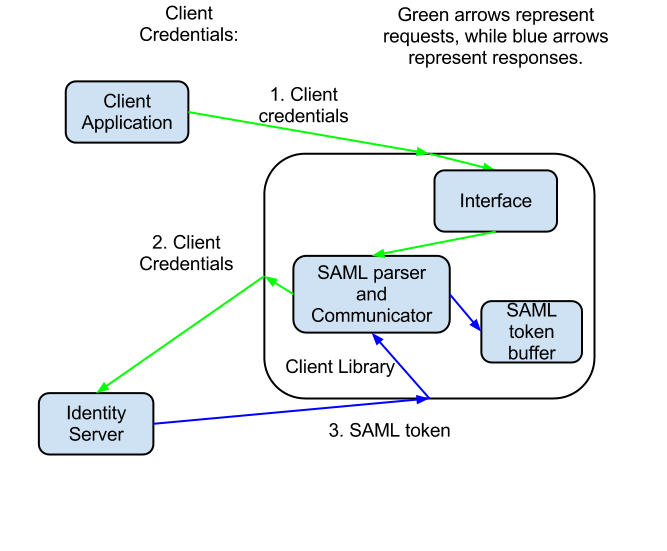
\includegraphics[width=\textwidth]{ClientCredentialsDataFlowDiagram}
        \caption{Client Credentials Flow}
        \label{fig:ClientCredentialsDataFlowDiagram}
    \end{figure}
    
    \begin{figure}[h]
        \centering
        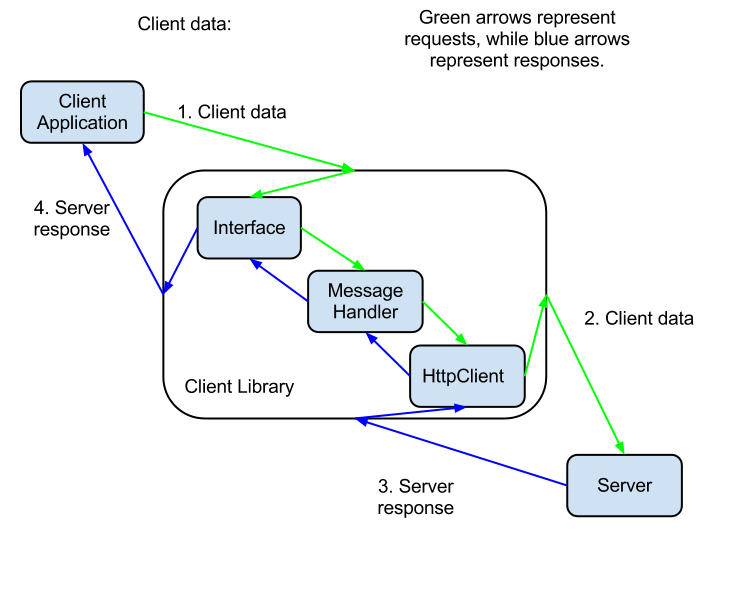
\includegraphics[width=\textwidth]{ClientDataFlowDiagram}
        \caption{Client Data Flow}
        \label{fig:ClientDataFlowDiagram}
    \end{figure}
    
    % the numbering on the figure and in the text does not match. This should maybe be fixed. 
		\textbf{Client credentials} (Visualized in Fig.\ref{fig:ClientCredentialsDataFlowDiagram})
		\begin{enumerate}
			\item From client application
			\item To client library via API/interface
			\item Via SAML to ID-server
			\item Back to client library as valid SAML-token
			\item Stored in library until client App changes credentials
		\end{enumerate}
		
	% The numbering on the figure and in the text does not match. This should maybe be fixed. 
		\textbf{Client Data} (Visualized in Fig.\ref{fig:ClientDataFlowDiagram})
		\begin{enumerate}
			\item Generated by client application
			\item Sent to client library via API/interface
			\item Buffered in library
			\item Sent from library to server
			\item Answer returned to client through library
		\end{enumerate}
		
	\subsubsection{Architecture}\label{client architecture}
		\begin{figure}[h]
			\centering	
			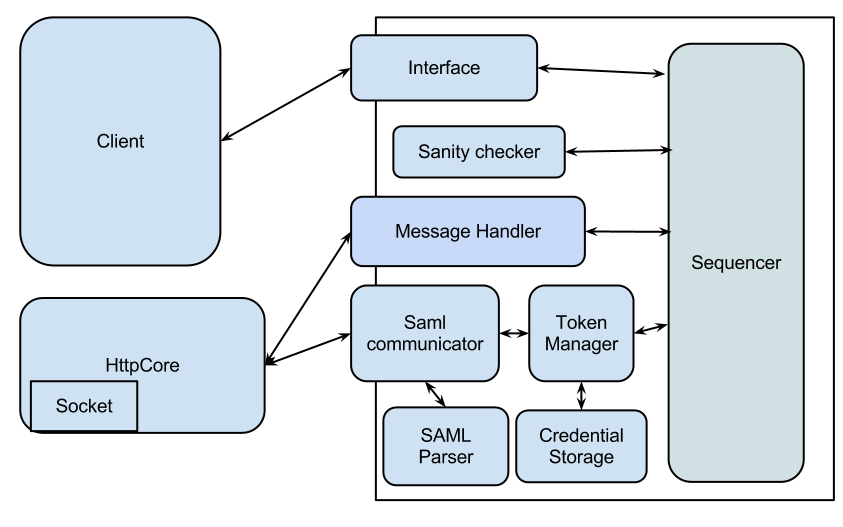
\includegraphics[width=\textwidth]{Detailedclientarchitecture}
			\caption{Detailed Client Architecture}
			\label{fig:DetailedClientArchitecture}
		\end{figure}

    All the following sub paragraphs in this subsection are parts of the client library wich Fig.\ref{fig:DetailedClientArchitecture}.  \\ 
    
		\indent \textbf{Interface} \\
Known in the class diagram as “QosClient”, responsible for providing a clean and easy to use interface for the clients.
\\\\
		\indent \textbf{Sequencer} \\
The central piece of the client library. Responsible for keeping a record of all other modules in the system and communicate between them as well as making sure everything happens in the right order.
\\\\
		\indent \textbf{Sanity checker} \\
	% todo: rewrite this section!
This module is simply there to do some easy verification of data that comes from the client, to make sure that it isn’t faulty in any obvious way (e.g: Data that isn’t xml, or credentials that are empty).
\\\\
		\indent \textbf{Token Manager} \\
This provides a nice and clean interface for the sequencer to store credentials and fetch tokens for data transmissions.
\\\\
		\indent \textbf{Saml Communicator} \\
This module will take care of the communication between the client library and the identity server.
\\\\
		\indent \textbf{Saml Parser} \\
This takes the reply from the identity server and parses it into a token object so that it can be easily used and stored.
\\\\
		\indent \textbf{Credential Storage} \\
Responsible for storing token objects as well as user supplied credentials. Also makes sure that no token objects are returned if they are invalid or expired.

	\subsubsection{Sequence Diagrams}\label{client sequence diagrams}
		\begin{figure}[H]
			\centering	
			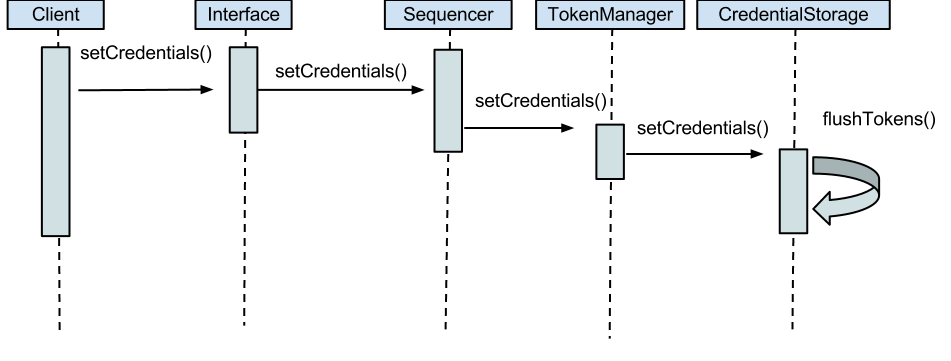
\includegraphics[width=\textwidth]{CliSeqDiaAcceptclientinfo}
			\caption{Accept client info}
			\label{fig:CliSeqDiaAcceptclientinfo}
		\end{figure}
		\begin{figure}[H]
			\centering	
			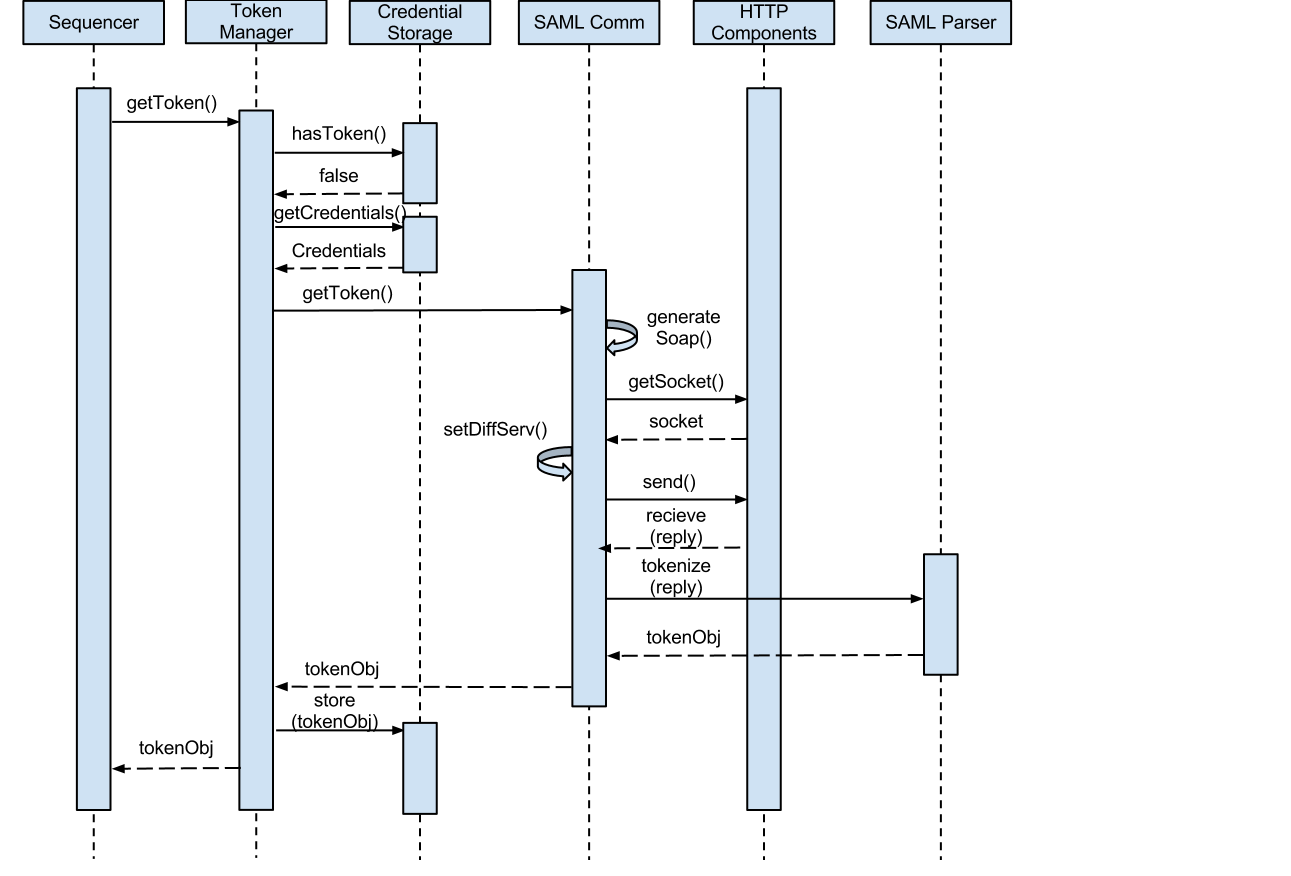
\includegraphics[scale=0.4, angle=-90]{CliSeqDiaGettingnon-storedtoken}
			\caption{Getting non-stored token}
			\label{fig:CliSeqDiaGettingnon-storedtoken}
		\end{figure}
		\begin{figure}[H]
			\centering	
			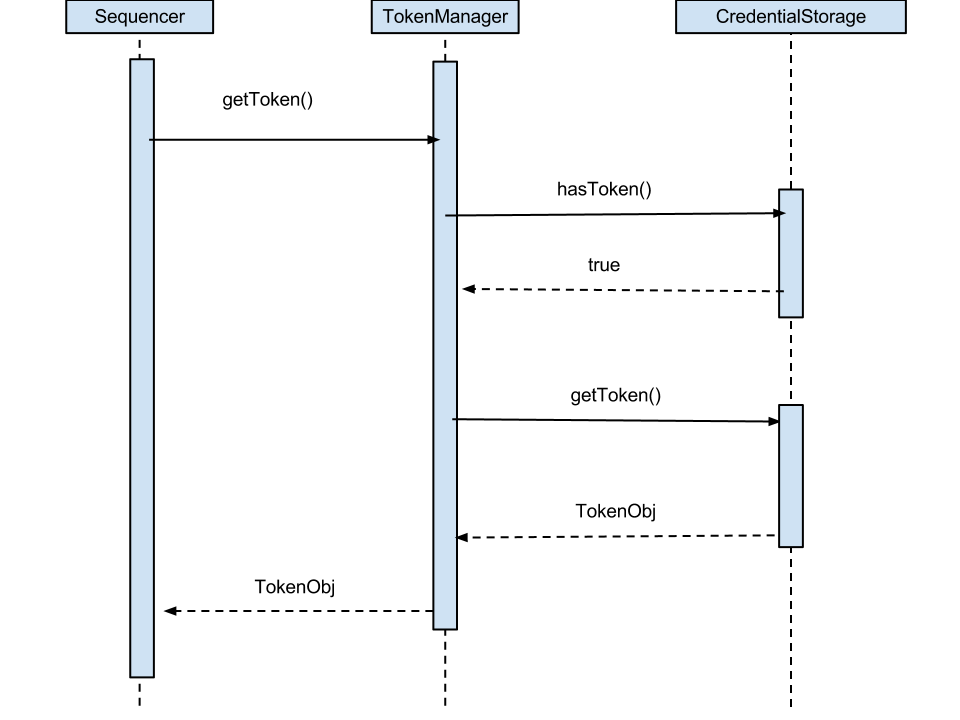
\includegraphics[scale=0.4, angle=-90]{CliSeqDiaGettingStoredToken}
			\caption{Getting stored token}
			\label{fig:CliSeqDiaGettingStoredToken}
		\end{figure}
		\begin{figure}[H]
			\centering	
			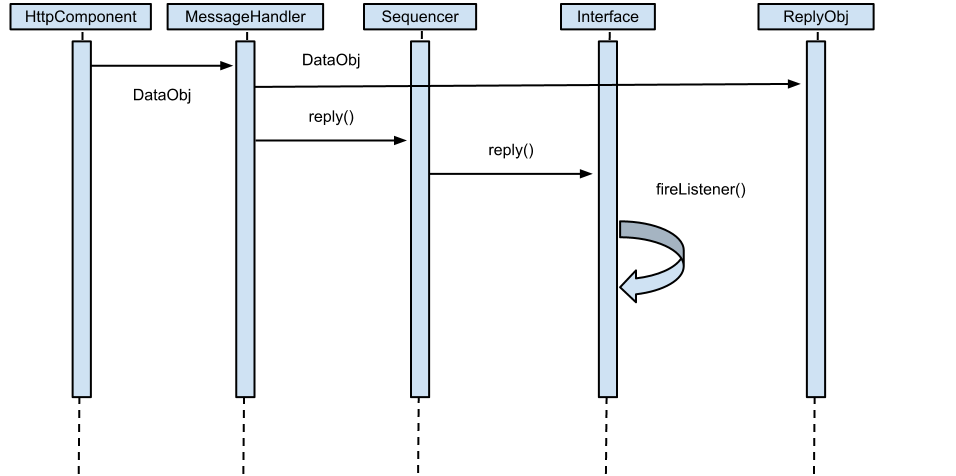
\includegraphics[scale=0.4, angle=-90]{CliSeqDiaReceivereply}
			\caption{Receive reply}
			\label{fig:CliSeqDiaReceivereply}
		\end{figure}
	% this sequence diagram might be better structured. Maybe with arrows happening first to be closes to echother. 
		\begin{figure}[H]
			\centering	
			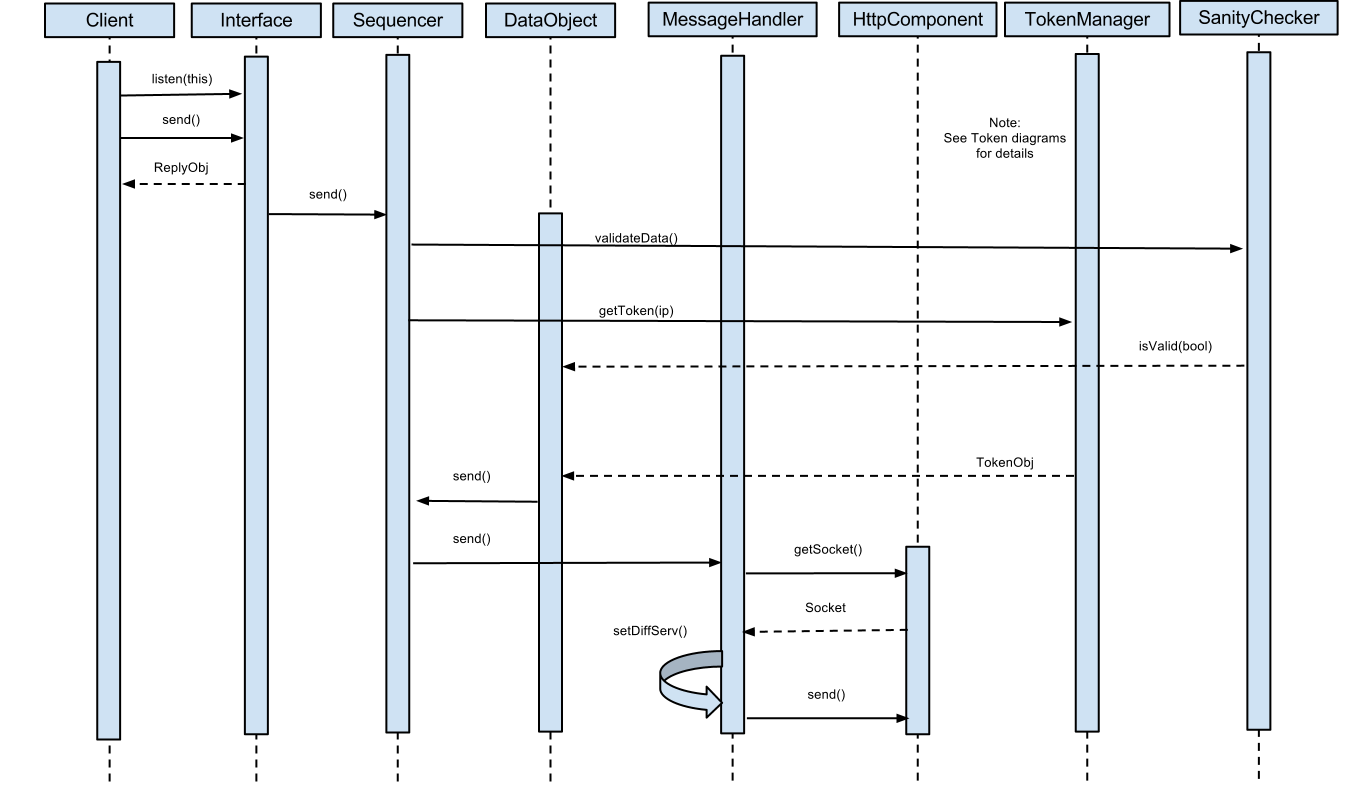
\includegraphics[scale=0.4, angle=-90]{CliSeqDiaSendData}
			\caption{Send data}
			\label{fig:CliSeqDiaSendData}
		\end{figure}

		


        \subsection{Server Side}\label{Server Side Design}

    In this chapter we are going to introduce the design, configuration and modification that we have done to the server side. In section \ref{Server Introduction} we will introduce the framework that we have built upon and what we are going to do with it. Next follows use cases, \ref{Server Use Cases}. Section \ref{Description of ESB concepts} will go into more detail about what the framework consists of. The section will also guide you through the basic processing units which is used in the framework. The next section, \ref{Textual Server Dataflow}, contains the dataflow through the server side, which will help you get a good overview of our thoughts about the design. \ref{Extensions to the ESB} goes into detail in describing our custom components in the framework, and together with the dataflow should give you a good understanding of the whole server side. Together with section \ref{Server Sequence Diagrams} you should get good system overview. Section \ref{Configuration of the ESB} will give you the 
details about how we have configured the framework, it will not contain description of how we have set variables during testing, but using this description should make it possible to get the framework up and running. The last section, \ref{Modification of the ESB} will depict how we have modified the framework to be able to meet our requirements, with this section you should be able to tell what modifications were needed and how we have altered those pieces. 

    \subsubsection{Introduction}\label{Server Introduction}
    The server side architecture consists of several components, the WSO2 ESB, the Monitoring Service and the GlassFish server. The GlassFish server is not necessary to modify and the MS is something we must assume exist in the network. The ESB is what we have to modify, configure and extend to meet our requirements.

    The ESB will be used to implement QoS for the web services. To do this, it will have to communicate with the MS, in addition to the clients and the services. The ESB must be configured to work as a proxy for the services on the GlassFish server. It will also be configured to use certain mediation sequences for incoming requests and outgoing responses. The extensions to the ESB consists mainly of custom mediators used in the mediation sequences. These mediators will have the tasks of determining priority of messages, contacting the MS for bandwidth data, and enforcing the priority. There will also be made modifications to one of ESB's library source code to allow setting the DiffServ field in the IP header.
    
    \subsubsection{Use Cases}\label{Server Use Cases}
    This section will outline the use cases that we have thought of in relation to the server side. With the help of these you should get a rough idea of what we want the server side to be able to do.\\\\
    \textbf{Title:} Request mediation\\
    \textbf{Requirements:} 3, 7\\
    \textbf{Actors:} Client, ESB, GlassFish\\
    \textbf{Main}
    \begin{enumerate}
        \item Client sends SOAP message with SAML Token to ESB proxy
        \item ESB extracts SAML token to get the client role
        \item ESB removes SAML metadata from message
        \item ESB adds metadata to message context.
        \item ESB sends message to GlassFish endpoint
    \end{enumerate}
    \textbf{Extensions:}
    \begin{itemize}
        \item[] 2a. SAML Token is invalid
        \item[] 2b. ESB sends error message to client
    \end{itemize}
    \textbf{Precondition:}
    \begin{itemize}
        \item Client is connected to ESB
    \end{itemize}
    ~\\
    \textbf{Title:} Response mediation \\
    \textbf{Requirements:} 2, 3, 7\\
    \textbf{Actors:} Client, ESB, GlassFish \\
    \textbf{Main}
    \begin{enumerate}
        \item GlassFish sends message to ESB
        \item ESB sets priority metadata in message context and SOAP header.
        \item ESB retrieves bandwidth information (See Monitoring Service communication use case)
        \item ESB prioritizes message (See Prioritize message use case)
        \item ESB sends message to Client
    \end{enumerate}
    \textbf{Extensions:} \\
    \textbf{Precondition:}
    \begin{itemize}
        \item Request mediation
    \end{itemize}
    ~\\
    \textbf{Title:} Monitoring Service communication\\
    \textbf{Actors:} Monitoring Service(MS), ESB\\
    \textbf{Main}
    \begin{enumerate}
        \item ESB requests bandwidth information from MS to a specific address
        \item MS returns bottleneck bandwidth to the ESB, as well as the address of the last Tactical Router before the endpoint.
    \end{enumerate}
    \textbf{Extensions:}
    \begin{itemize}
        \item[]	1a. ESB specifies an invalid address
        \item[]	2a. MS returns no information
        \item[]	2b. Address is in the same sub net as the ESB
    \end{itemize}
    \textbf{Precondition:}
    \begin{itemize}
        \item Response mediation
    \end{itemize}
    ~\\
    \textbf{Title:} Prioritize messages\\
    \textbf{Requirements:} 2, 6, 8\\
    \textbf{Actors:} ESB\\
    \textbf{Main}
    \begin{enumerate}
        \item ESB acquires QoS information through settings
        \item ESB adds QoS information to the SOAP header of the message
        \item ESB sets DiffServ field in IP header
    \end{enumerate}
    \textbf{Extensions:}\\
    \textbf{Precondition:}
    \begin{itemize}
        \item Response mediation
        \item Monitoring Service communication
    \end{itemize}

    \subsubsection{Description of ESB concepts}\label{Description of ESB concepts} 

    In this section we will shortly describe some important concepts of the ESB and message mediation.

    A mediator is the basic processing unit in \gls{synapse}\footnote{\gls{synapse} - An enterprise service bus}. Each message going through the ESB gets mediated through a sequence of mediators, which can be configured through either XML or WSO2’s graphical user interface. As long as the mediator inherit from a Synapse interface, any custom mediator can be used in the same manner as the built in mediators. To control the flow of messages through the ESB, there are two paths that can be controlled, the “in sequence” and the “out sequence”, which can also be configured to only apply for certain endpoints.

    The ESB is built around the notion of a message context, this object contains all the information regarding the message and the context around it. In the message context we can add properties, manipulate the message itself and manipulate the sending streams of the message. All the properties added during the receiving of a message is also added to the outgoing message, which we can use to our advantage.

    Each mediator in the sequence get access to the message context of the incoming or the outgoing message and can thus manipulate the context to its liking. When the mediator is done with the work it is supposed to do, it either calls the next mediator, sending it the possibly altered message context or returning true to indicate that the work is done.
    
    As you will soon see, we have taken full advantage of the modularity in the ESB. This means that even though much of the functionality in our mediators could be moved into one or two mediators we have decided to make many. For us this means much easier testing of each component and it gives each mediator a better defined role. For our customer this means an easier setup where they can mix and match each mediator and easily create custom sequences with just the functionality they need.

    \subsubsection{Dataflow}\label{Textual Server Dataflow} 
        This section describes the data flow through the ESB with the help of two diagrams. As a bonus, these diagrams show the general architecture of the server side very well.
\\
        \begin{figure}[h]
            \centering
            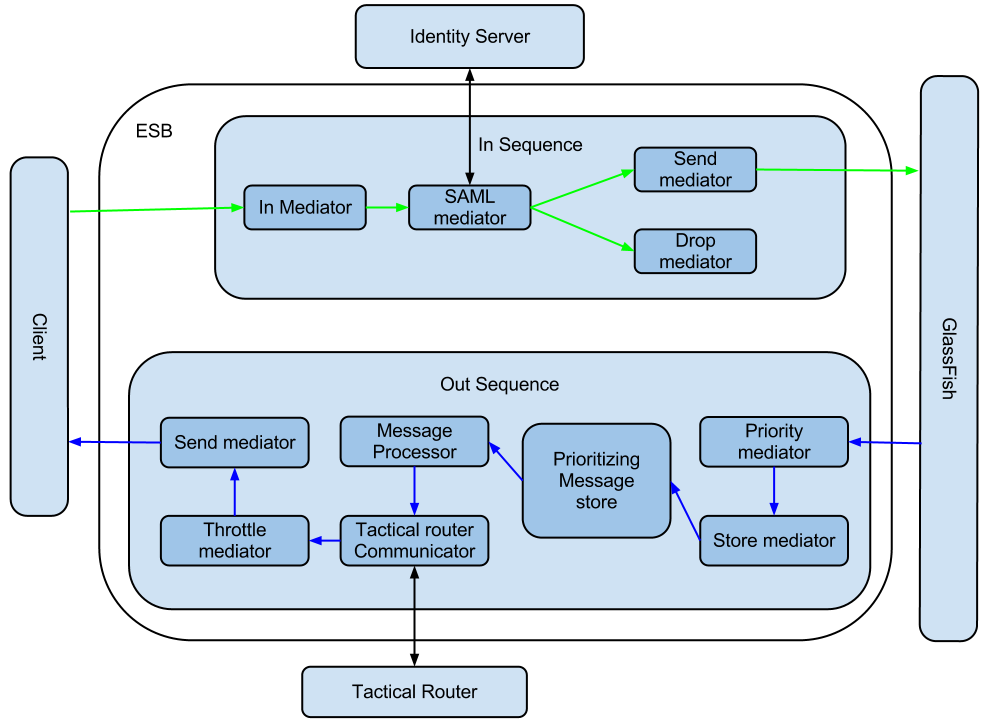
\includegraphics[width=\textwidth]{DataFlowDiagramServer}
            \caption{Server Data Flow}
            This diagram displays how the date flows through the server side. 
            \label{fig:DataFlowDiagramServer}
        \end{figure}
\\
Service Request :\\
To follow this flow, follow the green arrows in figure \ref{fig:DataFlowDiagramServer}. The ESB receives a request message from a Client, it is then sent to the SAML mediator, and then to the InMetadata mediator which when done sends it to the service endpoint on the GlassFish server, and the flow is over.
\\\\
Service Response:\\
To follow this flow, follow the blue arrows in figure \ref{fig:DataFlowDiagramServer}. The ESB receives a response message from the Service, it is then sent through a sequence of mediators, first the OutMetadata mediator, SoapPriority mediator, MS mediator and then  the Store mediator. The Store mediator stores the message in the Prioritized Message Store. The message is stored until the Sampling Message Processor picks it out before sending it on to another sequence of mediators. First in the sequence is the DiffServ mediator, then the Throttle Mediator and finally the Send mediator. The send mediator sends the message back to the client and the flow is completed.
\\
    \begin{figure}[h]
        \centering
        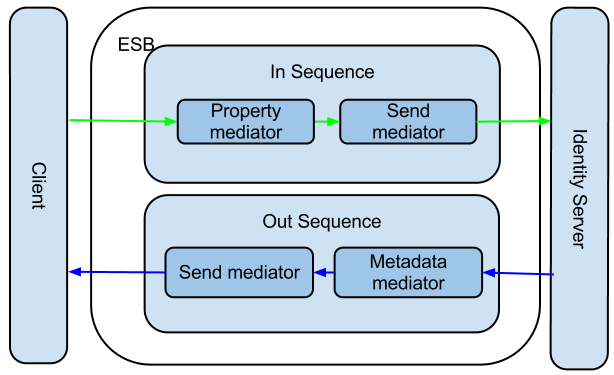
\includegraphics[scale=0.5]{SAMLauthenticationflow}
        \caption{SAML Authentication Flow}
        This describes the flow of an authentication request. 
        \label{fig:SAMLauthenticationflow}
    \end{figure}
\\           
SAML Authentication Request:\\
This flow is shown in figure \ref{fig:SAMLauthenticationflow}.The ESB receives a request (from a Client) directed at the dummy Identity Server, the ESB then uses the SendBack mediator to send the same message it got in back. The message then travels to the Out sequence where it gets a priority, a DiffServ value and some metadata gets added to the header of the message. The reason why this is done is explained in the section [TODO: Add reference to Identity Server problems here].%TODO fix

    \subsubsection{Extensions to the ESB}\label{Extensions to the ESB} 
    This section will contain a textual description of all the mediators used in the ESB. First we will describe all the custom mediators and then a short description of the built-in mediators we will use. All of our custom mediators have an accompanying sequence diagram to give a detailed overview of their inner working.
\\\\
\textbf{Custom mediators:}\\\\
SAML mediator:\\
    This mediator retrieves the user role from the SAML authentication and set this as a property in the message context. The service is retrieved from the 'recipient' field also found in the SAML authentication and added as another property. Depending on the configuration of the ESB this mediator can also detach the SAML authentication if this is no longer needed.
\\\\
InMetadata mediator:\\
	This mediator adds the IP of the client to the message context, which is done in order for the MS mediator to do its work. It will also set the Time-to-Live values in the message context if this is present in the SOAP header.
\\\\
OutMetadata mediator:\\
    This mediator retrieves the client role and service properties from the message context. These properties are then used along with a persistent registry to infer a priority for the message, and what the DiffServ field in the IP header should be set as. The priority and DiffServ values are then set as new properties in the message context.
    The DiffServ property in the message context will be used in the synapse core to set the DiffServ field before sending the message (See \ref{Modification of the ESB}).
\\\\
SoapPriority mediator:\\
	This mediator adds the DiffServ value and the priority as two custom SOAP header items. We use these fields on the client side in order for the clients to use the same DiffServ value.
\\\\
MS mediator:\\
    This mediator retrieves the \gls{ipaddress}\footnote{\gls{ipaddress} - A numerical label assigned to each device connected to the Internet} of the receiving client from the endpoint reference in the message context. It sends this IP address to the Monitoring Service and gets the IP address of the last Tactical Router on the path to the client, as well as the limiting bandwidth on the path. The mediator then sets this information as properties in the message context before sending the message to the next mediator.
\\\\
Prioritized Message store:\\
    This is not a mediator, but it is an important part of the response mediation sequence. This is a message store that stores messages in a priority queue. The queue is mainly ordered by the priority property of the message context, and secondly by the time when added. When retrieving messages from this store, the message on the top of the queue is returned. This ensures that high priority messages are processed before lower priority messages.
\\\\
DiffServ mediator:\\
	The DiffServ mediator sets the correct DiffServ value on the Socket. The DiffServ value is retrieved from the same value as the OutMetadata mediator put in earlier. Since correct use of DiffServ was very important to the client this mediator also does extensive logging which is important to look at when debuging.
\\\\
Throttle mediator:\\
    This mediator is used to ensure that high priority messages are sent first, by disrupting already sending messages, and it tries to ensure that the network is not being overflowed by this server by holding back messages. To determine what to disrupt and what to hold back, and for how long, several properties are used; the priority of the message, the available bandwidth, the IP address of the client side Tactical Router, and the real time demand of the request. In order to do this, the mediator must keep a list of sending messages and where those messages are going.
\\\\
SendBack mediator:\\
    This mediator sends the message back to the client, but before it is sent it is mediated through the out sequence of the ESB.
\\\\
\textbf{Built in Mediators:}\\\\
Send mediator:\\
    This is a built in mediator that sends the message to an endpoint (the requested service).
\\\\
Store mediator:\\
    This is a build in mediator that stores the message context in a message store, here this is the Prioritized Message store.
\\\\
Sampling Message Processor:\\
    This is not a mediator. It is a built in class that takes messages out of the Prioritized Message Store at a defined interval. And then sends them to a mediator sequence, here starting with the DiffServ mediator.

    \subsubsection{Sequence Diagrams}\label{Server Sequence Diagrams}
    This section contains some sequence diagrams which you can use to get a more in depth look into the code and methods used in the mediators above. The diagrams may not reflect the actual method names or display the full complexity of the code, but they should be sufficiently detailed that it should be possible to recognize them in the code.
    
        \begin{figure}[H]
        % TODO: ref in text. 
            \centering
            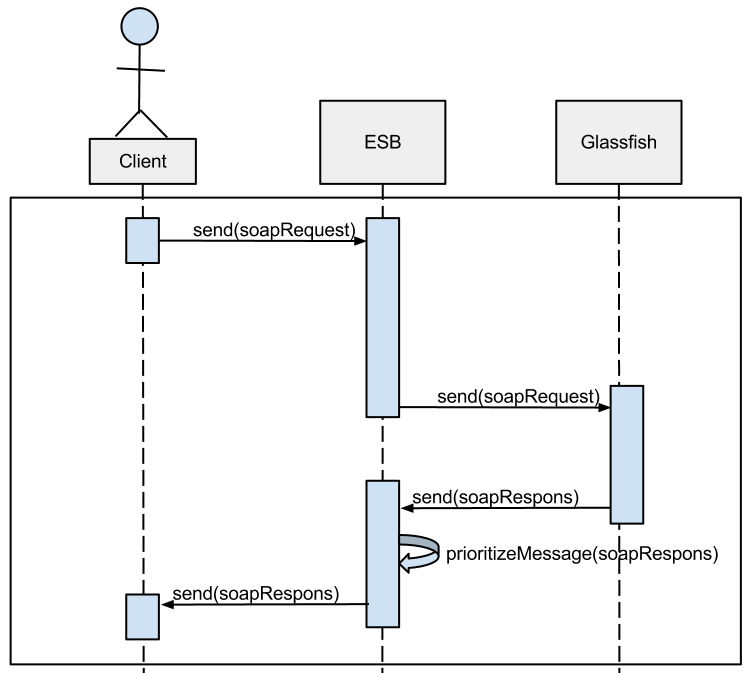
\includegraphics[scale=0.3]{System-levelsequencediagram}
            \caption{System-level sequence diagram}
            This high level diagram shows how the client communicates with web services through the ESB.
            \label{fig:System-levelsequencediagram}
        \end{figure}
        
        \begin{figure}[H]
        % TODO: ref in text 
            \centering
            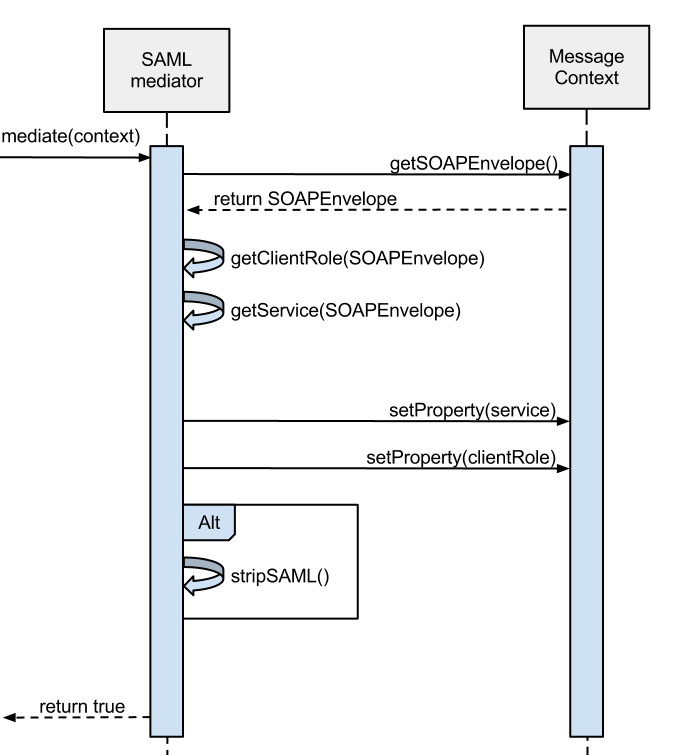
\includegraphics[scale=0.3]{SAMLmediator}
            \caption{SAML mediator sequence diagram}
            This diagram describes how the SAML mediator will get data from the message, and set it in the message context so it can be used later in the response sequence
            \label{fig:SAMLmediator}
        \end{figure}
        
        \begin{figure}[H]
        % TODO: ref in text 
            \centering
            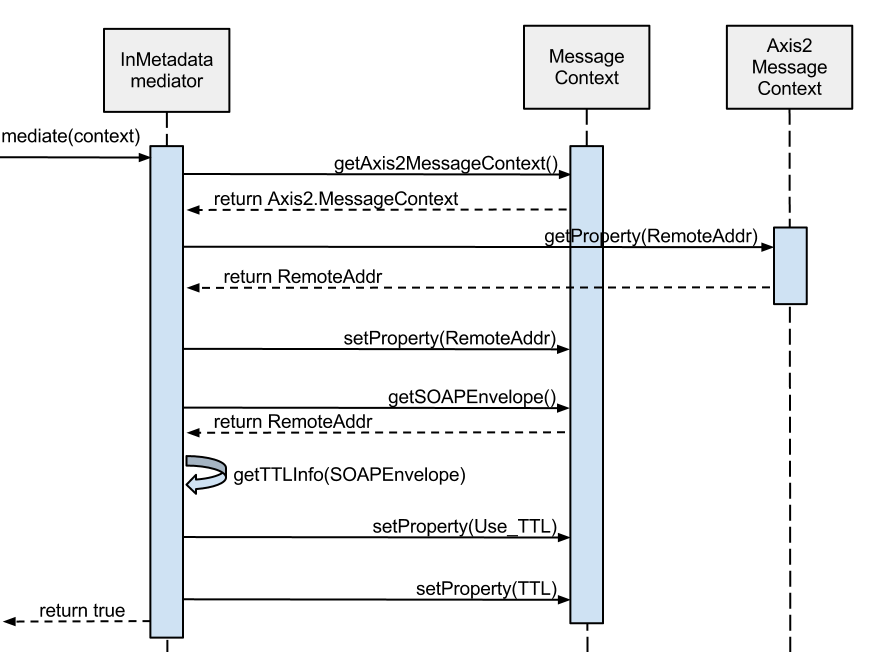
\includegraphics[scale=0.3]{InMetadatamediator}
            \caption{InMetadata mediator sequence diagram}
            This diagram shows how the InMetadata mediator works when it adds the IP address and Time-to-Live.
            \label{fig:InMetadatamediator}
        \end{figure}
        
        \begin{figure}[H]
        % TODO: ref in text. 
            \centering
            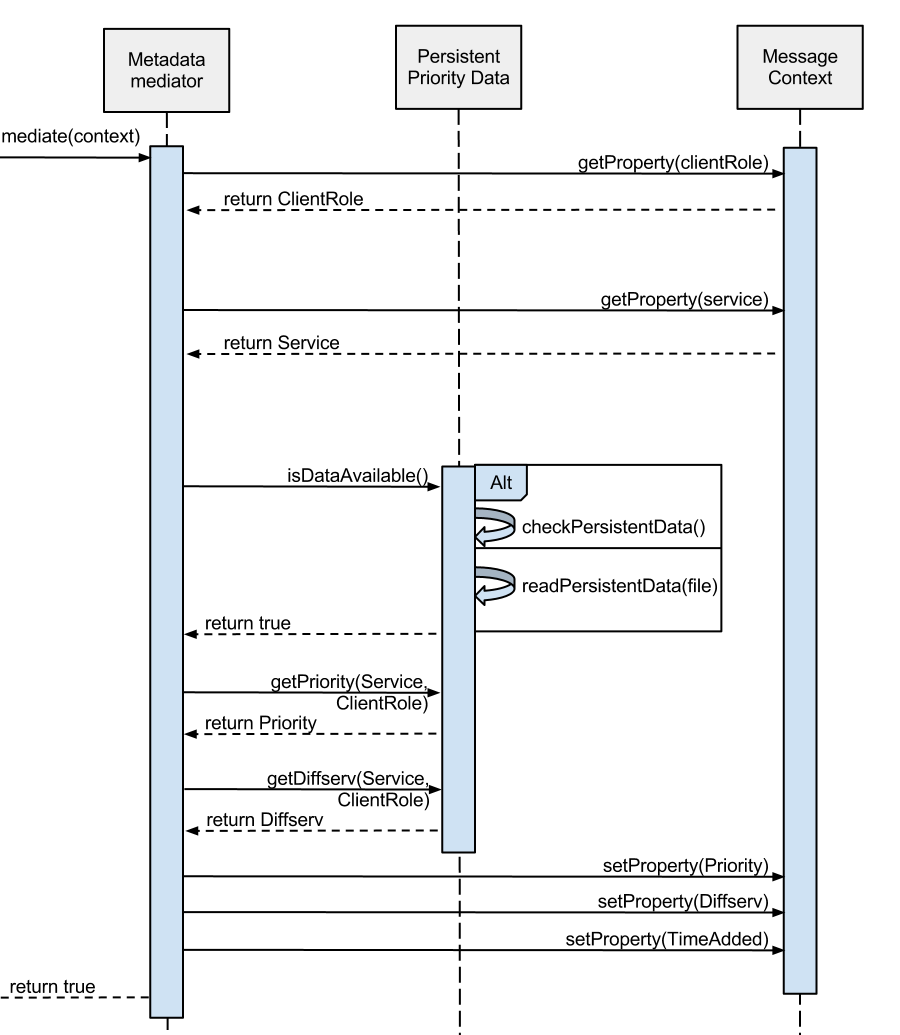
\includegraphics[scale=0.4]{OutMetadatamediatorsequencediagram}
            \caption{OutMetadata mediator sequence diagram}
            The diagram shows how OutMetadata mediator works.
            \label{fig:OutMetadatamediatorsequencediagram}
        \end{figure}
        
        \begin{figure}[H]
        % TODO: ref in text 
            \centering
            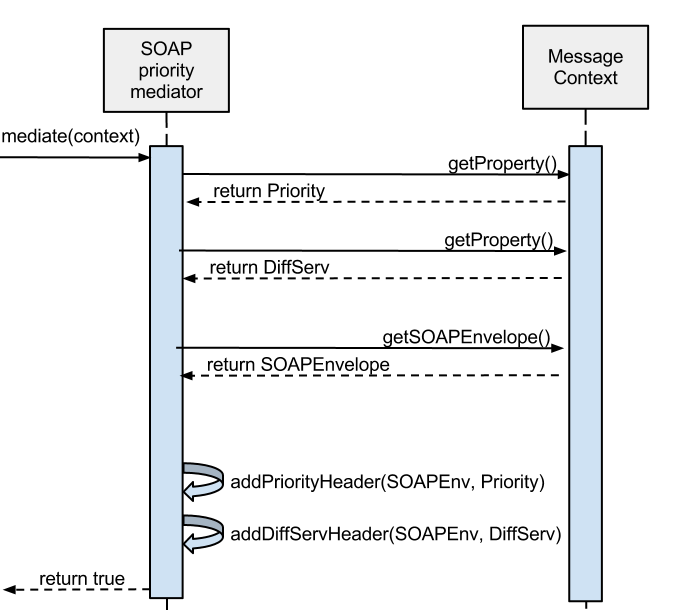
\includegraphics[scale=0.3]{SoapPrioritymediator}
            \caption{SOAP Priority mediator sequence diagram}
            This diagram shows the inner working of the SOAP priority mediator.
            \label{fig:SoapPrioritymediator}
        \end{figure}
    
        \begin{figure}[H]
        % TODO: ref in text. 
            \centering
            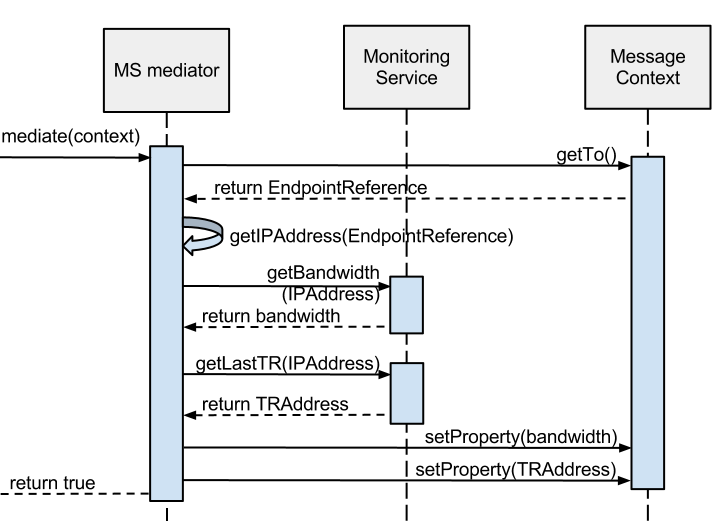
\includegraphics[scale=0.3]{MSmediatorsequence}
            \caption{Metadata mediator sequence}
            This diagram describes how the Metadata mediator retrieves previously stored properties from the message context, determines a priority for the message, and sets priority and DiffServ properties in the message context
            \label{fig:MSmediatorsequence}
        \end{figure}
        
        \begin{figure}[H]
        % TODO: ref in text 
            \centering
            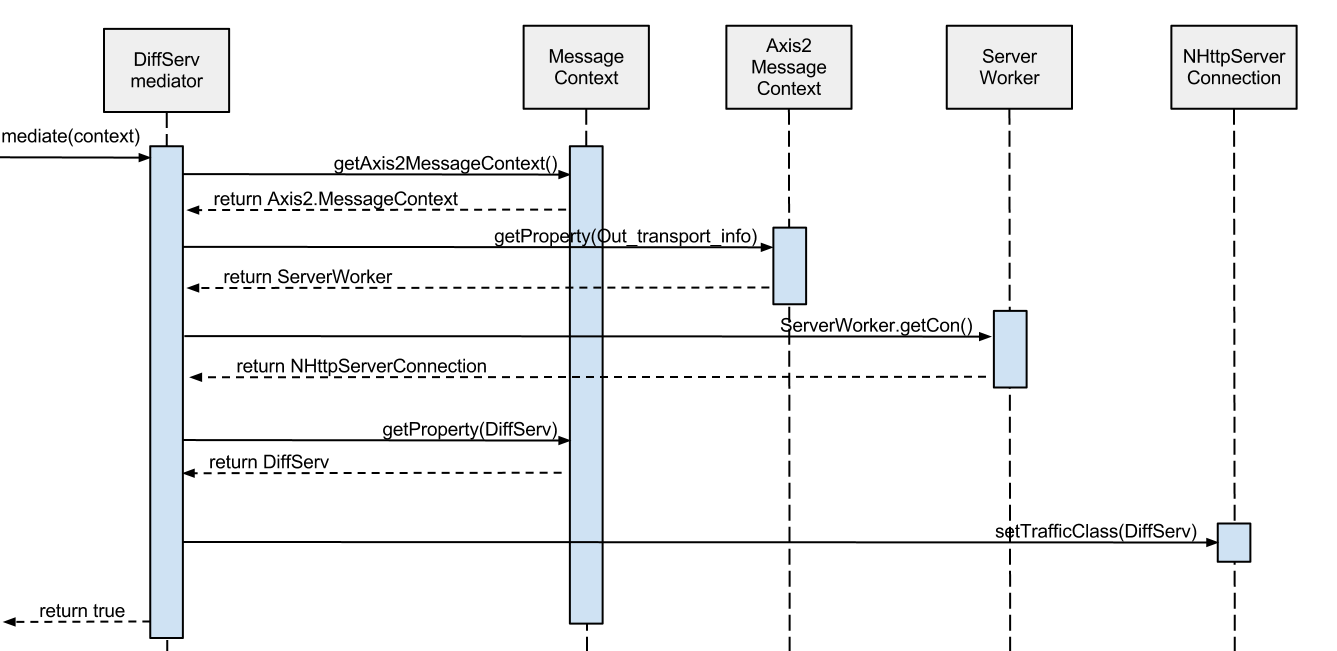
\includegraphics[scale=0.3]{DiffServmediator}
            \caption{DiffServ mediator sequence diagram}
            How we set DiffServ priority on the underlying Socket.
            \label{fig:DiffServmediator}
        \end{figure}
        
        \begin{figure}[H]
        % TODO: ref in text 
            \centering
            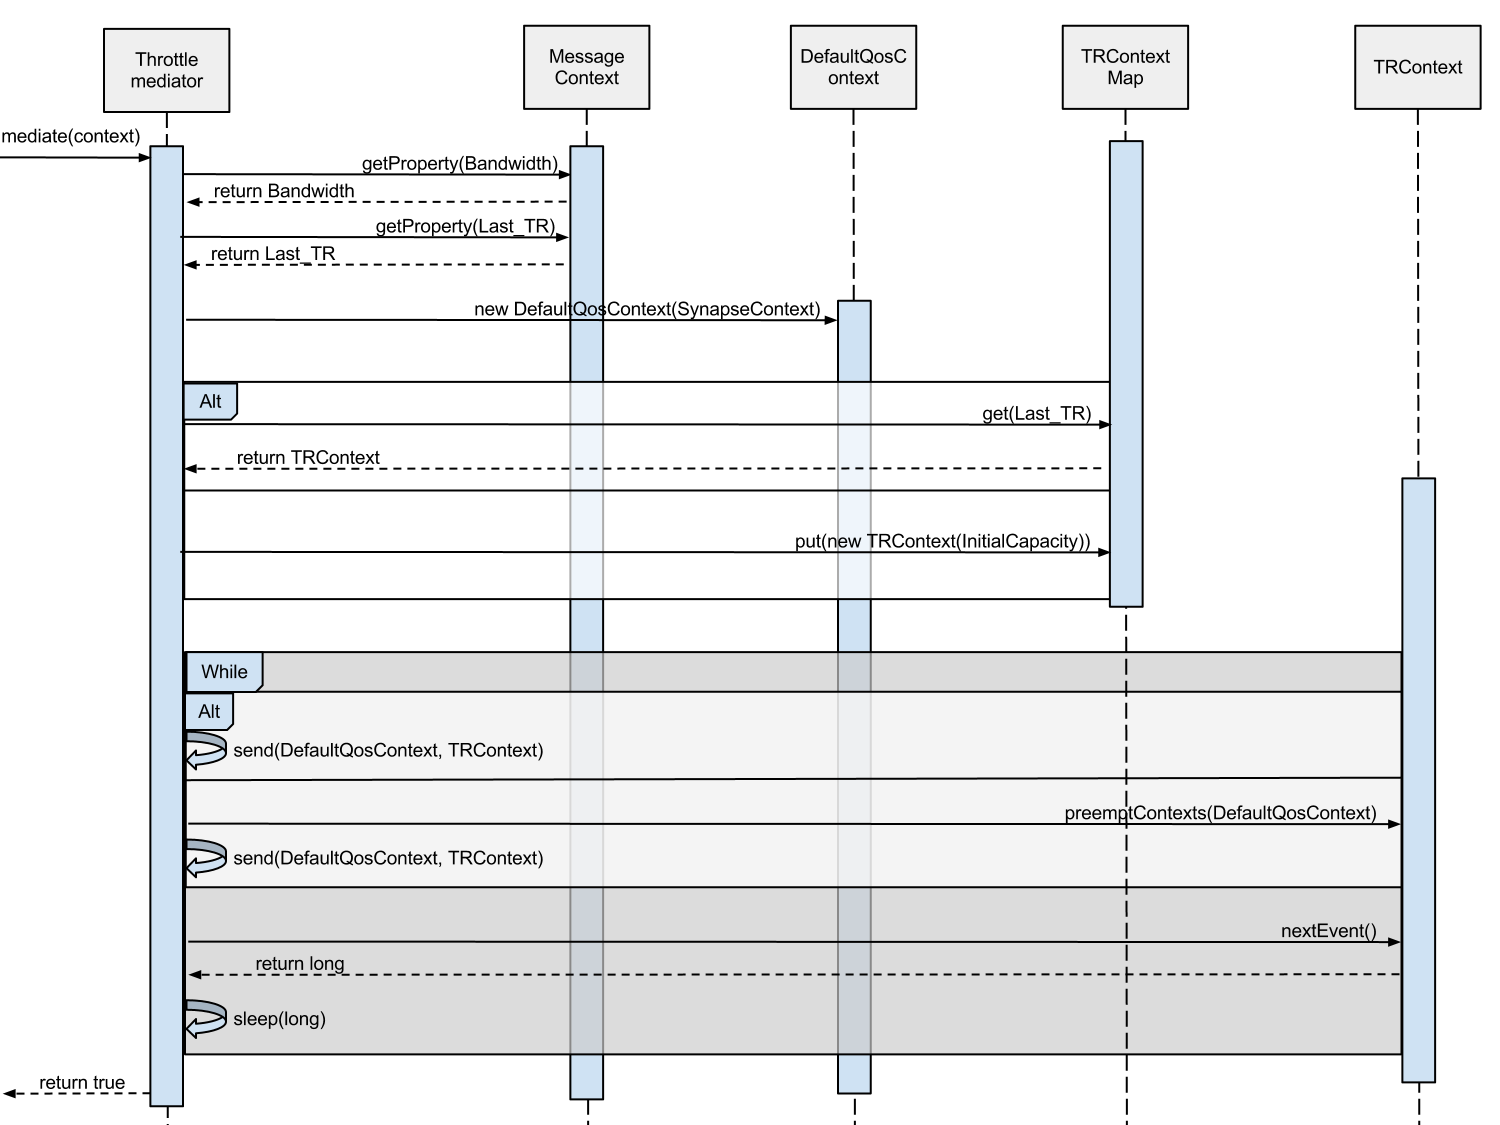
\includegraphics[scale=0.3]{Throttlemediator}
            \caption{Throttle mediator sequence diagram}
            The meat of the server side mediators.
            \label{fig:Throttlemediator}
        \end{figure}
        

    \subsubsection{Configuration of the ESB}\label{Configuration of the ESB} 
	In this section we will explain how to configure the ESB. For general configuration of the ESB, f.ex. configuring new services or WS-Discovery, please refer to the official WSO2 ESB or Apache Synapse documentation.

	\begin{shaded}
	It is highly recommended that you follow the appendix [TODO: add reference to appendix] for an in depth guide on how to setup the ESB with the needed modifications before you read this section.
	\end{shaded}

	First we will look at the file “ppd.xml”, which should now be in “/path/to/wso2esb/”, ppd is short for Persistent Priority Data. This file contains maps from “service name” and “client role” to “priority” and “diffserv”. Here “service name” should be the path to the service on the ESB, “client role” should be the name of the client’s role, “priority” is the internal priority we use in the ESB (higher is better) and “diffserv” is the value that will be set in the IP header on communications with the client. Both DiffServ and priority must be integers.
	The service element also has the useDefault property, which when set to true lets roles not configured in this file use values in the default role. When useDefault is set to false unconfigured clients will get a priority and DiffServ of 0. If useDefault is set to false there is no need to configure a default client for the service.
	Below is an example setup of a service in ppd.xml.\\

\lstset{language=XML}
\begin{lstlisting}[frame=single] %Ok to not have this referenced =)
<?xml version="1.0" encoding="UTF-8" ?>
<config>
   <services>
	   <service name="/services/EchoService" 
	   useDefault="true">
	         <client role="clientRole1">
	           <priority>100</priority>
	           <diffserv>10</diffserv>
	         </client>
	       <client role="Default">
	           <priority>321</priority>
	           <diffserv>8</diffserv>
	       </client>
	   </service>
   </services>
</config>
\end{lstlisting}\\

	Next we look at a file that is specific to our implementation of the MSCommunicator (Monitoring Service Communicator). Since our implementation does not actually have a monitoring service to contact we use the file “ms.xml” in “/path/to/wso2esb/” to configure data groups of destination IP, name of last Tactical Router before client and the bandwidth capacity of the ‘weakest’ link on the path measured in KBps. Below is an example configuration.\\

\lstset{language=XML}
\begin{lstlisting}[frame=single] %It is ok that this is not referenced in text =)
<?xml version="1.0" encoding="UTF-8" ?>
<config>
   <RoutingInfos>
	   <RoutingInfo>
	       <destIP>127.0.0.1</destIP>
	       <lastTR>bob</lastTR>
	       <bandwidth>0.2</bandwidth>
	   </RoutingInfo>
   </RoutingInfos>
</config>
\end{lstlisting}\\

	If the MSCommunicator is modified to communicate with a Monitoring Service this file will not be needed anymore.

	The last file we will look at is synapse.xml (\ref{attachment:server config}), which should now be in “/path/to/wso2esb/repository/deployment/server/synapse-configs/default/”. This file contains configuration for proxies, endpoints, message stores, mediation sequences, and more. The important things here are:
	\begin{itemize}
	\item the sequence qos, where we can find the configuration for the Throttle mediator. Here we can set the properties minBandwidthPerMessage (integer measured in Bps) as well timeout, which is the longest time a message will be allowed to try sending (integer measured in ms) before it is discarded.
	\item and the messageProcessor, where the parameter interval can be set, this determines how often a message should be taken out of the message store, measured in ms.
	\end{itemize}
	Other things in this file should mostly be untouched, as they define what the ESB does with messages, most of which is needed to do the prioritizing and throttling.

	The ESB can also be configured through its web interface on https://ADDRESS:9443/carbon

    \subsubsection{Modification of the ESB}\label{Modification of the ESB} 
		The WSO2 ESB source code will have to be modified to allow for setting the DiffServ field in the IP-header of packets sent. The idea is that we will set a property, DiffServ, in the message context, and let the DiffServ mediator retrieve this property and set it on the socket used for sending.

The source code for all the dependencies of WSO2 ESB is included in its source code. As such we only altered files in this source. This made it easier for us to build and create a runnable instance of WSO2’s ESB. To also try and support future versions of Apache Synapse and WSO2 we have also pushed the changes upstream, which should mean that in the future WSO2 will support setting DiffServ by default.    

    
    \subsection{Changes}\label{Changes}
        There are a lot of changes from the initial prestudy design to the final design described in this chapter. The prestudy design did not go into a lot of detail because of limited knowledge about the systems we were to be using. Some assumptions made proved to be wrong, and a lot of difficulties popped up along the way. We had a very long planning phase before the implementation in this project. Before we started the implementation we were much closer to the final design than we were in the prestudy, with only a few notable changes made during implementation. These changes are what we would like to discuss in this chapter. This discussion should help you get a better understanding of some of our discoveries, and maybe why we ended up with the product we now have.
     

   \subsubsection{Server Changes}\label{Changes:Server}
    

   \subsubsection{Server Specific Changes}\label{Changes:Server}
    On the server side there was not a lot of big changes during the implementation.
    
    The biggest change from early design to final design is probably the ThrottleMediator. Before we started the implementation, we were very unsure of what we would be able to do in this mediator. So we wrote down a few things we wanted to try, most of which we managed to implement. We wanted to make it more dynamic, and maybe learn something from how long data took to be sent to the different endpoints. Time was a limited resource, but we ended up making more out of it than what was initially anticipated.

    Initially OutMetadataMediator did the work of SoapPriorityMediator as well, but we split them up because we figured several more specialized mediators would be more modular and easier to modify later.

    During implementation we found out that we had to get the IP address of the client in the 'in' sequence for use later in the 'out sequence, so we made InMetadataMediator take care of this as well as getting potential time to live data.

    Because of the lack of the Identity Server we needed an alternative to send the diffserv value back to the client. So we made the SAML-sequence described in section ~\ref{Description of ESB concepts} under SAML Authentication Request.
\subsubsection{Changes that affect both sides}\label{Changes:both}
\\\\
OpenSAML:\\
OpenSAML is not used at all. If we had succeeded in implementing the Identity Server, the IS would take care of all SAML generation. Since we use a dummy layer in the ESB to “simulate” the IS, the client needs to generate SAML, but it takes far too much time to initialize the OpenSAML libraries for it to be useful in our case, so we decided not to use it, and instead use Apache Axiom to build a proper SOAP-wrapped SAML-message based on some hardcoded strings, and variable roles and timestamps.
\\\\
Tokens:\\
The biggest change since the initial design finalization is how tokens are fetched and used in our implementation. The initial idea was that the server side would contain an identity server, which our client would identify itself towards. As it turned out, setting up and using the identity server was a near impossible task (see details on why below) that would have taken us far beyond our project deadline, so together with the customer it was decided that since this wasn't a part of the requirements for the project, it could be dropped. What we ended up with was a far simpler system where the client itself creates a token, which is then sent to a simple echo service on the server to get the SOAP headers we needed from it.\\

\subsubsection{Regarding the Identity Server}\label{Changes:IS}

Our original design called for the implementation of the WSO2 Identity Server, but our final product does not include it as we ran into some problems while trying to set it up. After discussing our situation with the customer, they agreed that we could drop it. It was, after all, not a functional requirement from their side, though it would be preferable to have it included.

    There are several reasons why we failed to implement the Identity Server, one of which is that we started our research of the IS too late, only two weeks before our prototype demonstration, and we only had one group member working on it. After seeing how well documented and fairly easy to use the WSO2 ESB was, we figured that the IS couldn't be much worse, but we figured wrong. Which leads us to the next source of our problems; the WSO2 Identity Server product page at \url{http://wso2.com/products/identity-server} is severely lacking in documentation. The user guide and administration manual contains barely no information about how to configure it and set it up to be usable in different usage scenarios. They provide links to some blog posts that employees had written back in 2009, and even though the blogs contained some useful information, and sometimes provided example configuration files and client code, they did not state which versions of the different products they were basing their examples on, so we don't know if there were compatibility problems between different versions of the IS and ESB.

    We used this blog post \url{http://blog.facilelogin.com/2009/05/accessing-proxy-services-in-wso2-esb.html} to try and set up communication between the IS and ESB. It was not entirely similar to our use case, as it uses X509 signing and encryption with HTTP transport, instead of using HTTPS and let the transport layer take care of security. When we tried to use the supplied client code and configuration files, we got some problems with the latter, as the client code would not accept them, throwing exceptions stating that they were not of the correct format, though the IS and the ESB accepted them. If we changed the configuration files so that the client would accept them (the only adjustment needed was to change the name of a tag in the WS-security policy XML-file, from \textless sp:Policy\textgreater\ to \textless wsp:policy\textgreater) then the IS and ESB would not accept them. Since it was just a minor adjustment, and the rest of the policy stayed identical, we don't believe this caused any problems, but it is an example of how frustrating it could be trying to use the code provided, as it was poorly commented and assumed you had previous knowledge of how Apache Axis2, Axiom, Rampart and Tomcat worked, since the WSO2 IS builds upon these products.

    After much trial and error, a lot of exceptions and googling for solutions, we managed to get the IS to issue security tokens and send them to the ESB, but the ESB failed in decrypting and verifying them. We were unable to figure out exactly why it failed, as the error message we got was that the ESB could not find the public key of the Identity Server, but using the Java keytool we could verify that the key was in fact present in the ESB key store. After spending quite a few hours trying different solutions, exporting the IS public key and importing it to the ESB key store under a new alias, importing the ESB public key into the IS key store etc. we gave up, as this specific use case was not the one we were after, and we had at least succeeded in getting the ESB and IS to talk to each other.

    Next, we tried configuring the IS to issue username tokens and send them over HTTPS, which would remove the need for endpoint encryption and was after all the use case we had in mind. We could find no specific examples for this scenario, so we tried creating our own security, policy file, since the one from the previous example specified endpoint encryption, and adjusted the settings in the ESB and IS. In this way we managed to get the IS to create username tokens, but nothing more, as it crashed when trying to send it to the ESB, stating that the SOAP header did not include a security element. Monitoring the SOAP messages we could see that the header actually did contain this element, so we don't know why the IS couldn't find it.

    This was as far as we got before our prototype demonstration, and as already mentioned, our customer agreed that we could drop the Identity Server and instead use a dummy layer in the ESB. This means that our final product does not use the IS, and users cannot log on to the system because there is no user store, so the client will create static SAML-tokens which it sends to the dummy layer in the ESB, which then returns the same SAML-token, but wraps in in a SOAP message containing information about the clients priority in the system and its diffserv value.

    Had any of us had some experience with WS-security from before, and been familiar with the WS-security policy language, and the Axis2, Axiom, Rampart and Tomcat from Apache, which the WSO2 Identity Server builds upon,  we might have been more successful. We were quite frankly stumbling around in the dark, without knowing exactly where to begin.





